
En el trabajo desarrollado en la Universidad Tecnol\'ogica de Lanzhou en China
 \cite{Zhang2017},hacen un an\'alisis del comportamiento del soldador experto
 humano utilizando un sistema de inferencia neurodifuso adaptativo (ANFIS,
 por sus siglas en ingl\'es) para su automatizaci\'on, considerando las variables
 de los materiales usados y caracterizando la tarea del soldador humano.
 En la figura~\ref{fig:syswelding} se puede apreciar el sistema experimental
  resultante del proyecto mencionado.


\begin{figure}[h]
\centering
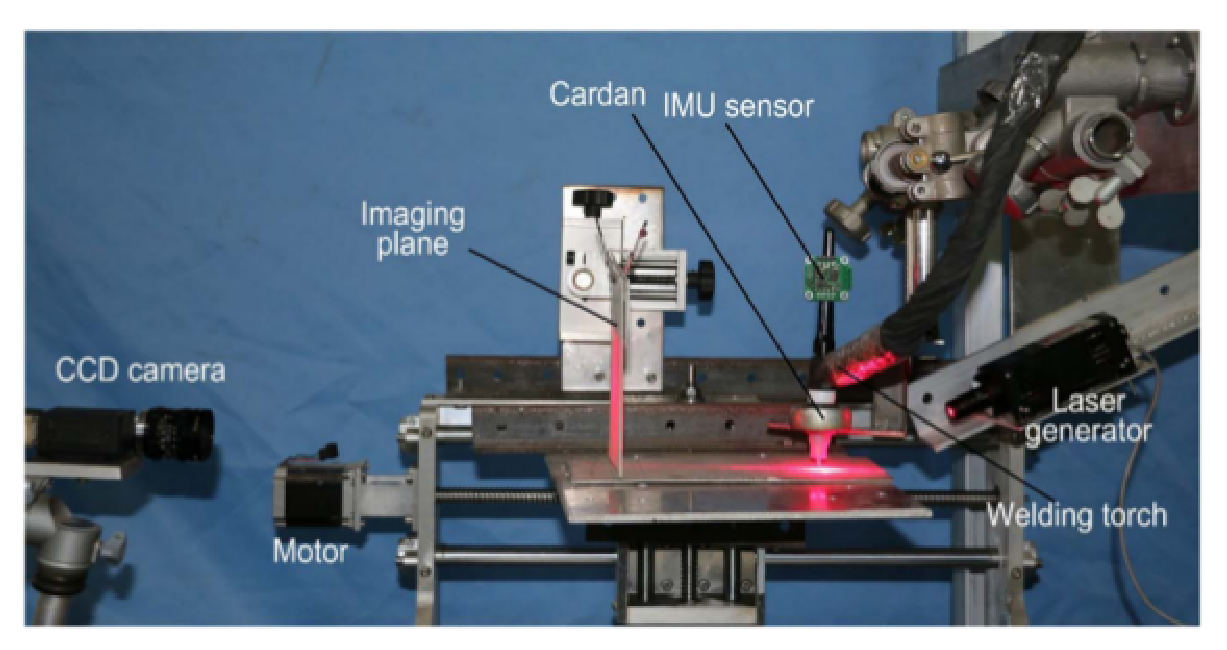
\includegraphics[width=0.8\columnwidth]{chap2/Imagenes/Welding.eps}
\caption{Sistema experimental de la soldadora.}
\label{fig:syswelding}
\end{figure} 
 